\documentclass[a4paper,twoside,10pt]{article}

\usepackage[USenglish]{babel}
\usepackage[T1]{fontenc}
\usepackage[ansinew]{inputenc}

\usepackage{lmodern}


\usepackage{graphicx}

\usepackage{amsmath}
\usepackage{amsthm}
\usepackage{amsfonts}
\usepackage{dsfont}


\begin{document}

\title{Mapillary Assignment}
\author{David Ok}
\maketitle

All implementations are in C++. This was not the best decision as it allowed to explore only a small number of ideas among those I had.

\section{Recurring Pattern Detection}

\subsection{Overview}
Image sequences in Mapillary presents recurring patterns we want to get rid off. This is a binary segmentation problem with a temporal dimension.

Our method is as follows. The user chooses a frame of an image sequence, typically the first one in our examples (but not necessarily). The user labels (i) parts of the image corresponding to streetview and (ii) uninteresting parts of the image he wants to get rid off as illustrated in Fig. \ref{fig:labeled_frame}.


\begin{figure}
	\centering
  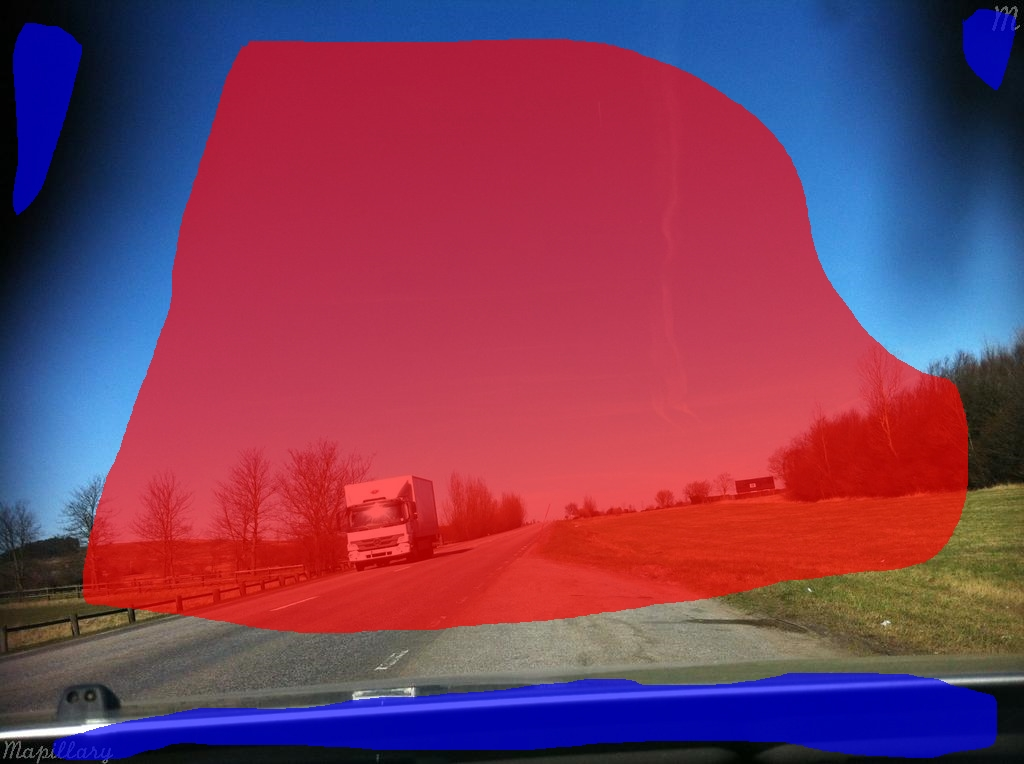
\includegraphics[width=0.8\textwidth]{labeled_frame.jpg}
	\caption{First labeled frame of a Mapillary sequence}
	\label{fig:labeled_frame}
\end{figure}

We adopt a graph-cut based segmentation approach by exploiting two prior knowledges:
\begin{itemize}
\item the color-based distribution of each class,
\item the temporal frequency of each label in each pixel.
\end{itemize}

A very brief summary of the approach is the following.
\begin{enumerate}
\item We label the remaining unlabeled pixels of the first frame will labeled based on the scribbles.
\item For the next images of the sequence, we update the color-based distribution and the temporal consistency distribution by using the previous segmentation results.
\item We craft an energy where the data term is constructed from the color-based prior and the temporal prior.
\item We minimize the energy using max-flow to segment the image (we use Kolmogorov's C++ implementation).
\end{enumerate}

\subsection{How to run the program}
Please see the \texttt{README.md} file in the repository.


\subsection{Approach}

This last method seems promising but much work remains to be done. Among the plethora of graph-cut based approaches, let us mention that the GrabCut algorithm is one of those approaches, which is available in openCV. Because of its iterative minimization approach, GrabCut is a little bit slow.

Here I choose to do a more basic graph-cut but this time by encoding more relevant prior knowledge.

In the sequel, we introduce some notations. let $0$ be the class of pixels we want to get rid off by and $1$ be the class of streetview pixels we want to keep. For a given time step $t$, we denote by:
\begin{itemize}
\item $\mathbf{I}_t$ the $t$-th image of the sequence;
\item $\mathbf{I}_t(p)$ the color of pixel $p=(x,y)$ in frame $\mathbf{I}_t$;
\item $l_{p,t}$ the label of pixel $p=(x,y)$ in frame $\mathbf{I}_t$;
\end{itemize}

For each image $\mathbf{I}_t$, we minimize the following energy

\begin{equation}
\sum_p g_{p,t}(l_{p,t}) + \sum_{p,q} h_{p,q,t} (l_{p,t}, l_{q,t})
\end{equation}

Note that $g_{p,t}$ and $h_{p,q,t}$ are respectively the data term and the regularization term and that they \emph{evolve} over time.


\subsubsection{Photo-consistency for the data term.}
Using the training data, we compute the following color-based prior distributions from the training data. From the training data, we compute:
\begin{itemize}
\item the histogram function $h(l = 1, \mathbf{c}) = \displaystyle\sum_{1 \leq p \leq N} \mathds{1}_{\{\mathbf{c}_p = \mathbf{c}\}}$, which counts the number of pixels with color $\mathbf{c}$ that with label $l=1$.
\item the histogram function $h(l = 0, \mathbf{c}) = \displaystyle\sum_{1 \leq p \leq N} \mathds{1}_{\{\mathbf{c}_p = \mathbf{c}\}}$, which counts the number of pixels with color $\mathbf{c}$ that with label $l=1$.
\end{itemize}
Then we renormalize the histogram to obtain color-based distributions $P(l = 1 | \mathbf{c})$ and $P(l = 0 | \mathbf{c})$, i.e., the probability that a pixel $p$ with color $\mathbf{c}$ is labeled with label $l=1$, respectively $l=0$.

Because we deal with an image sequence, we can update the histograms $h(l = 0, \mathbf{c})$ and $h(l = 1, \mathbf{c})$ at each time time step $t$. Since we have a temporal dimension, histograms are now denoted with a subscript index $t$ as $h_t(l = ., \mathbf{c})$.

Histogram functions are updated as follows. Let us just explain $h_{t}(l = ., \mathbf{c})$ is updated. Let a fixed label be $l=1$ (for example) and a fixed color $\mathbf{c}$, the histogram function is updated as follows:
\begin{equation}
h_{t+1}(l = 1, \mathbf{c}) = h_t(l=1, \mathbf{c}) + \sum_{p \in D} \mathds{1}_{\{l_{p,t+1} = 1\ \cap\ \mathbf{I}_{t+1}(p) = \mathbf{c}\}}
\end{equation}
In words, we add here the number of pixels in the frame $\mathbf{I}_{t+1}$ that are labeled $l=1$.

The color-based distributions $P_t(l = . | \mathbf{c} = \mathbf{c})$, which now evolves over time, are still obtained by renormalising the histogram functions $h_{t}(l = ., \mathbf{c})$.



\subsubsection{Temporal consistency for the data term.}
Most of the time, the uninteresting pixels, e.g. the car hood, which we want to remove are stationary. It is therefore relevant to count the number of times $T_t(p)$ a pixel $p=(x,y)$ has been labeled as $l=0$ from time steps $t'=1,\dots,t$.

The update rule is as follows:
\begin{equation}
T_{t+1}(p) = T_t(p) + \mathds{1}_{\{l_{p,t+1} = 0\}}
\end{equation}
In words, after segmenting the frame $\mathbf{I}_{t+1}$, we increment $T_{t+1}(p)$ if the label of pixel $p$ is $0$.

Then, we can compute the probability $f_t(p) = \frac{T_t(p)}{t}$ that pixel $p$ will be labeled $l=0$. Let's call it the temporal-consistency prior term.


\subsubsection{Data Term}
Using those two prior distributions, our data term is finally:

\begin{equation}
g_{p,t+1}(l_p) = \displaystyle \left\{\begin{array}{ccc}
-\log(P_t(l_p=0 | \mathbf{c}=\mathbf{I}_t(p))) & -\log(f_t(p)) & \text{if}\ l_p = 0 \\
\underbrace{-\log(P_t(l_p=1 | \mathbf{c}=\mathbf{I}_t(p)))}_{\text{photo coherence}} & \underbrace{- \log(1-f_t(p))}_{\text{temporal coherence}} & \text{if}\ l_p = 1 \\
\end{array} \right.
\end{equation}



\subsubsection{Regularization term.}
The regularization term is classical

\begin{equation}
h_{p,q,t}(l, l') = \displaystyle \left\{\begin{array}{cc}
0 & \textrm{if} \ l = l' \\
\lambda \frac{\exp(-\kappa \|\mathbf{I}_t(p) - \mathbf{I}_t(q)\|^2)}{\|p-q\|_2} & \text{otherwise}\\
\end{array}\right.
\end{equation}



\section{Experiments}

We show some results for the image sequence \texttt{-ywLysPFu3TL85zOMOYJkw} in Fig. \ref{fig:results}.

In our implementation, for the 5 first images of the sequences, we don't use the temporal prior but we keep updating it at each iteration. That is because we don't have enough data. Then, in the next frames, not only does the temporal prior helps to better estimate the recurring patterns but it also accelerates the max-flow computation.
In my machine, the 5 first frames were segmented in 1.5 seconds on average, and then the segmentation of the next frames were on average done in 0.7 seconds.

The segmentation results were done with the format 1024 x 764, that looks reasonably fast and the promising results encourages to craft better prior knowledge.


\begin{figure}
	\centering
  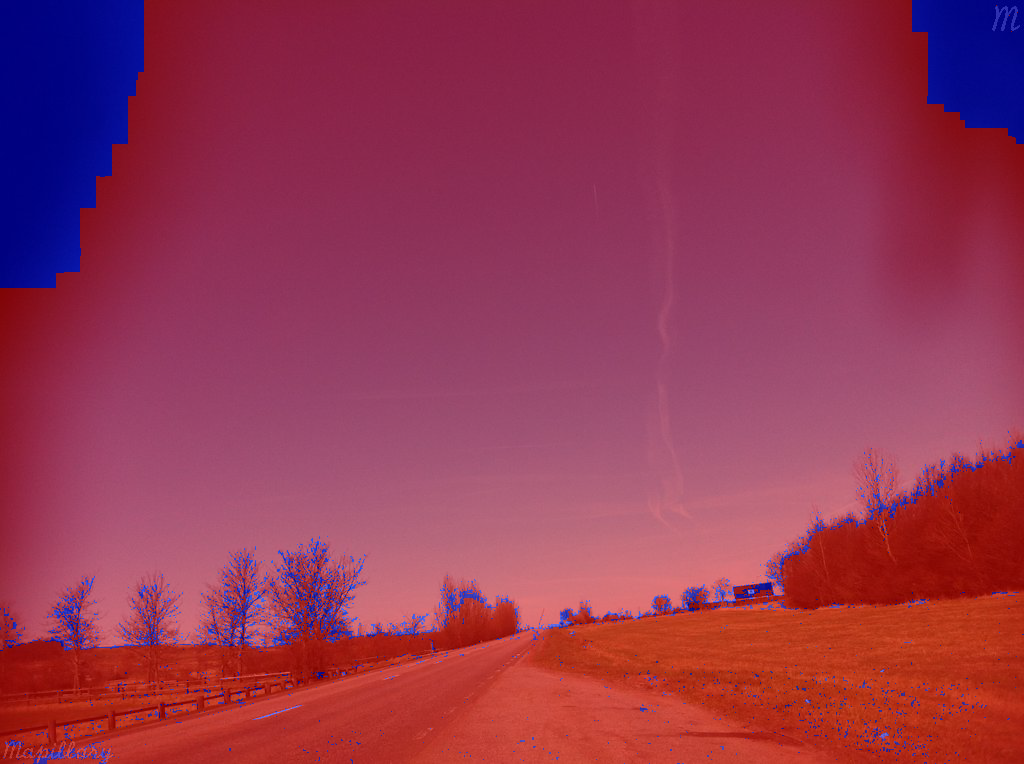
\includegraphics[width=0.45\textwidth]{result_1.png}\ 
  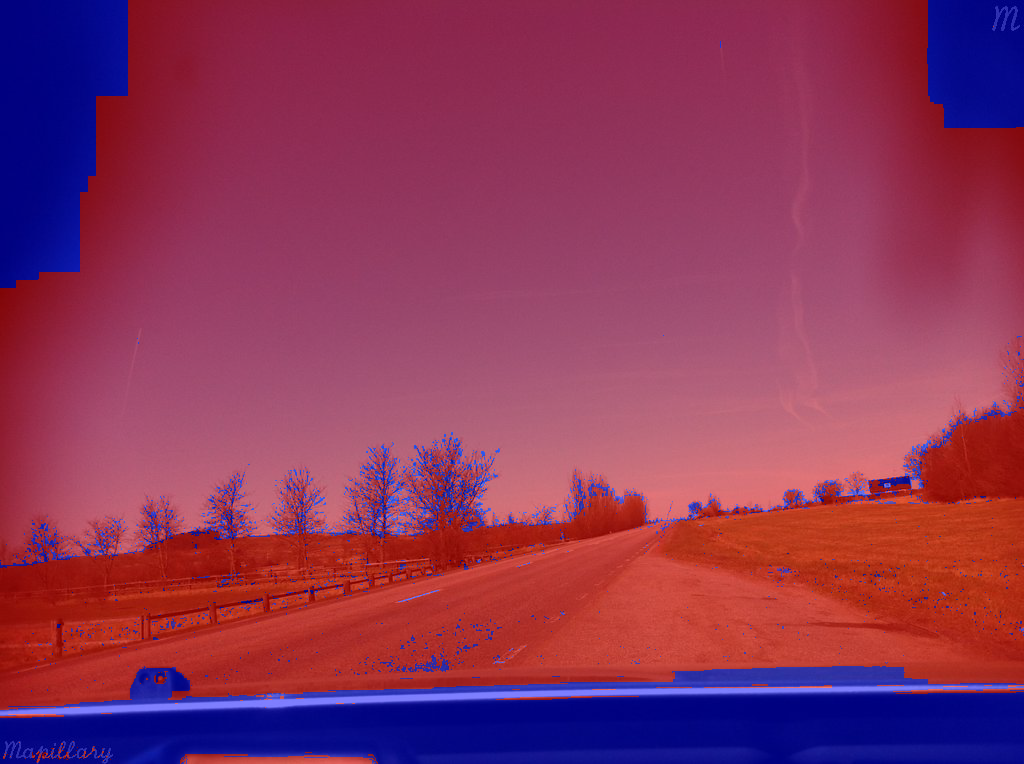
\includegraphics[width=0.45\textwidth]{result_3.png}\ 
  \\
  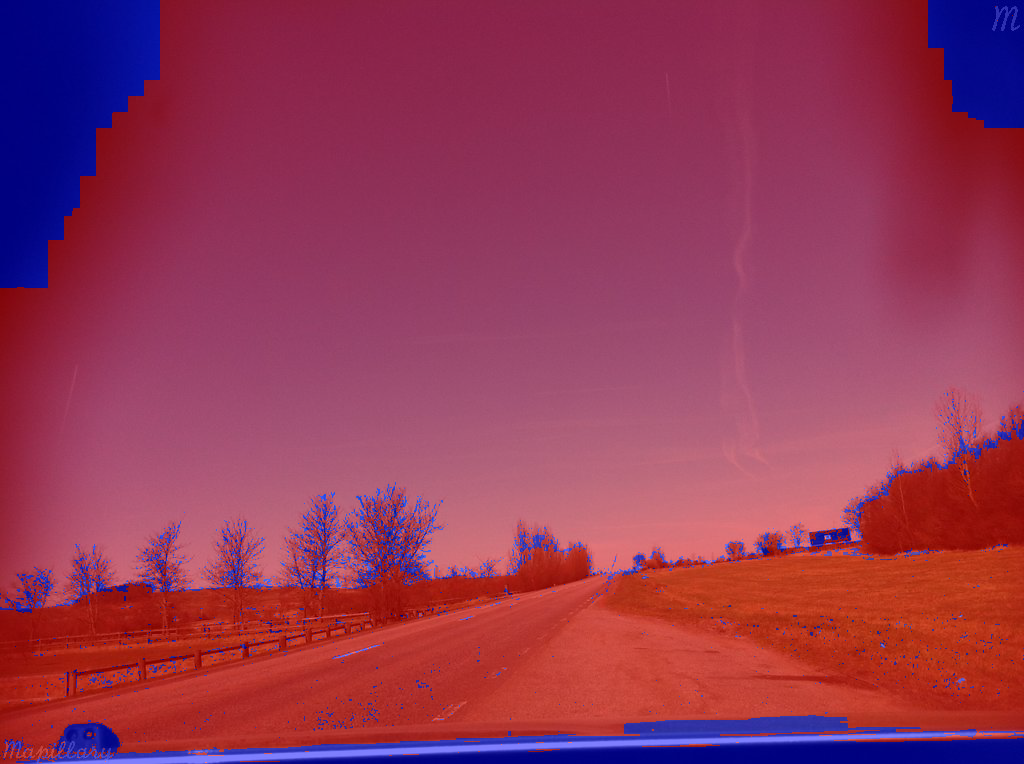
\includegraphics[width=0.45\textwidth]{result_5.png}\ 
  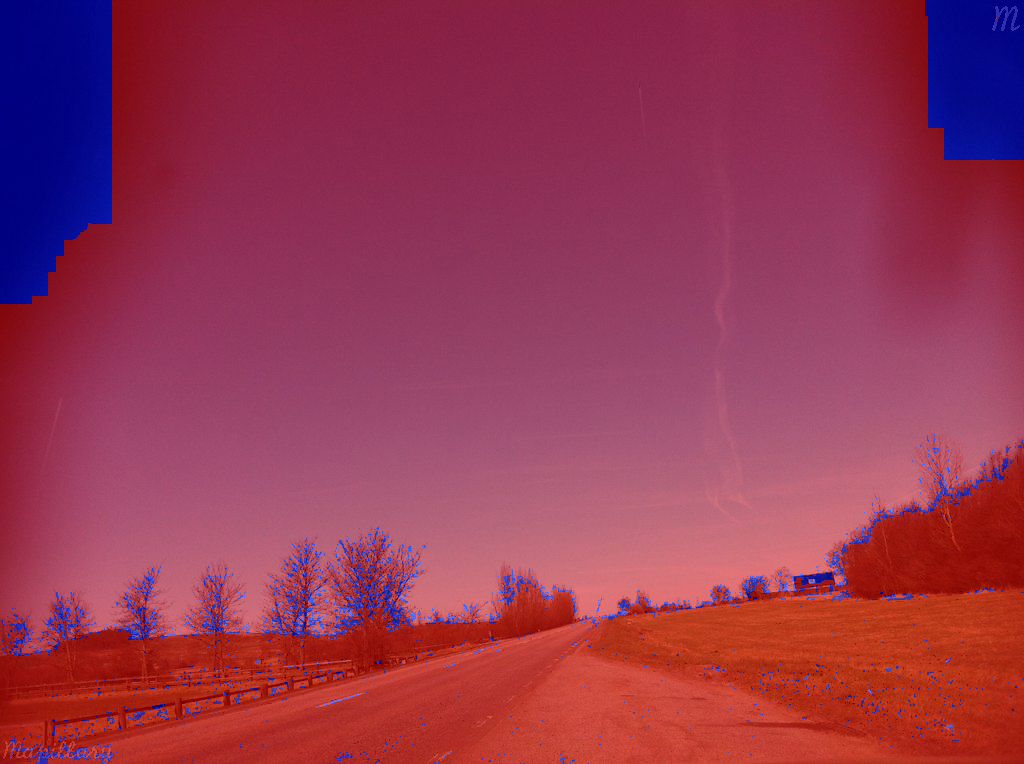
\includegraphics[width=0.45\textwidth]{result_7.png}\ 
  \\
  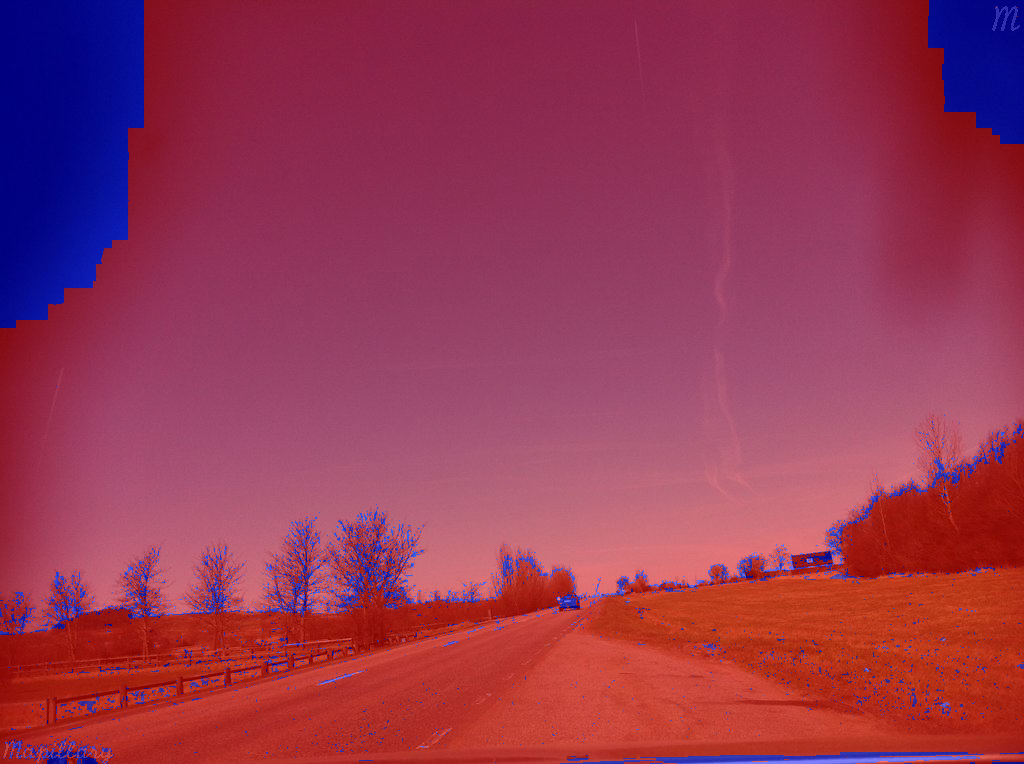
\includegraphics[width=0.45\textwidth]{result_9.png}
  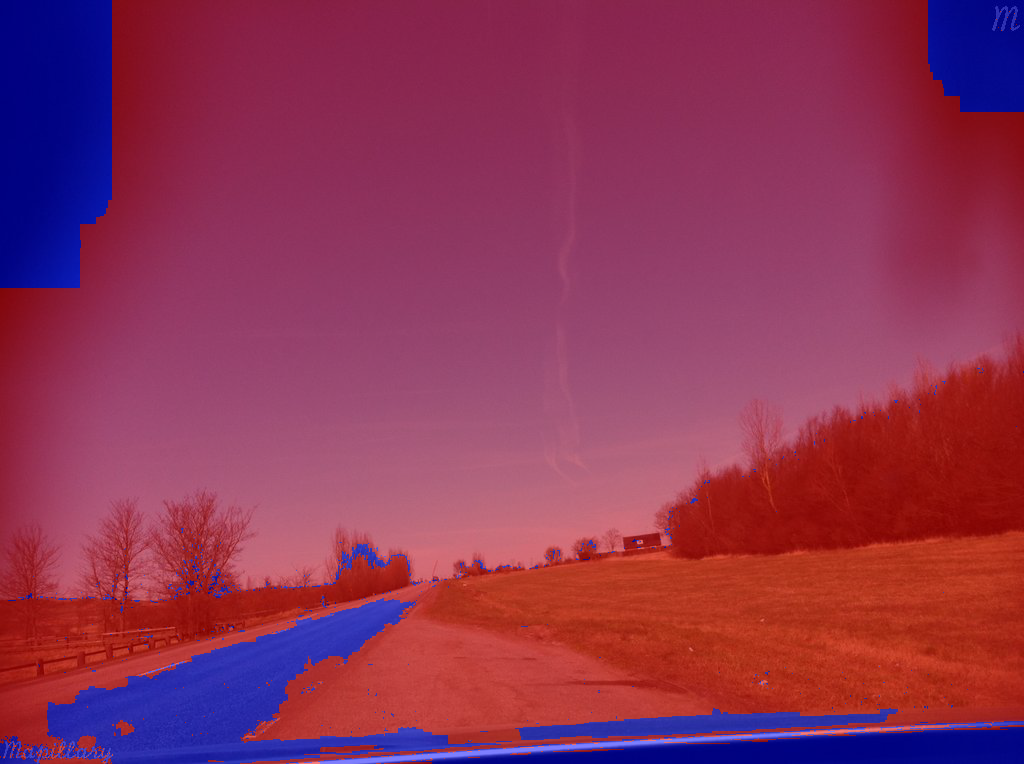
\includegraphics[width=0.45\textwidth]{result_11.png}
  \\
  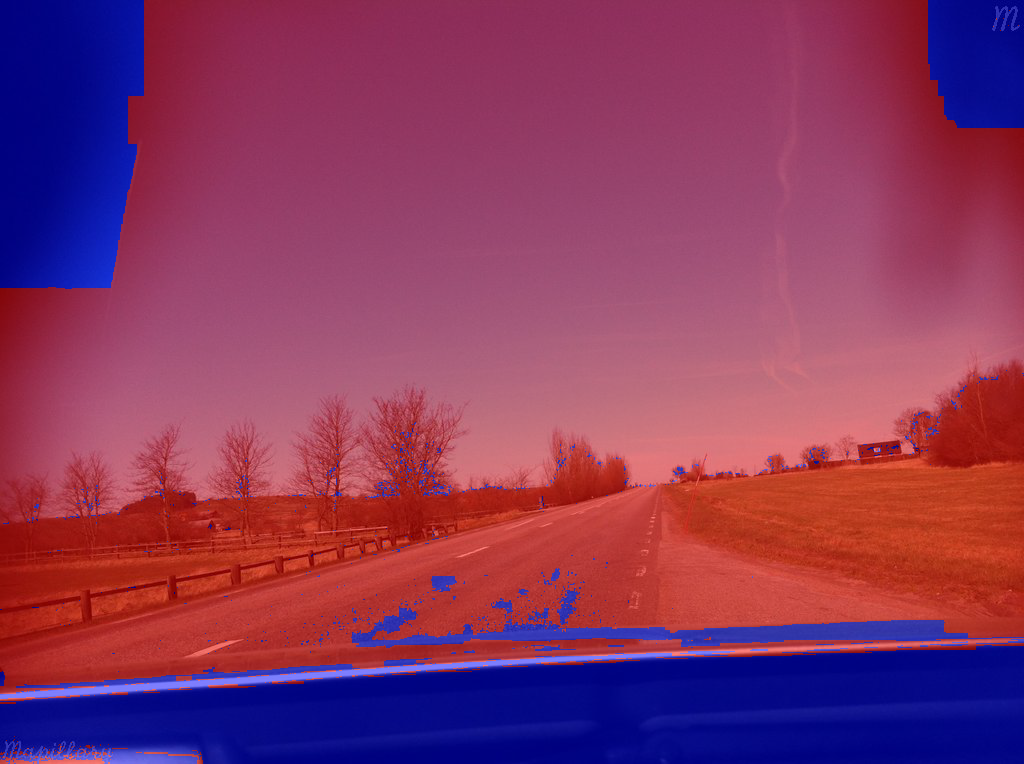
\includegraphics[width=0.45\textwidth]{result_13.png}
  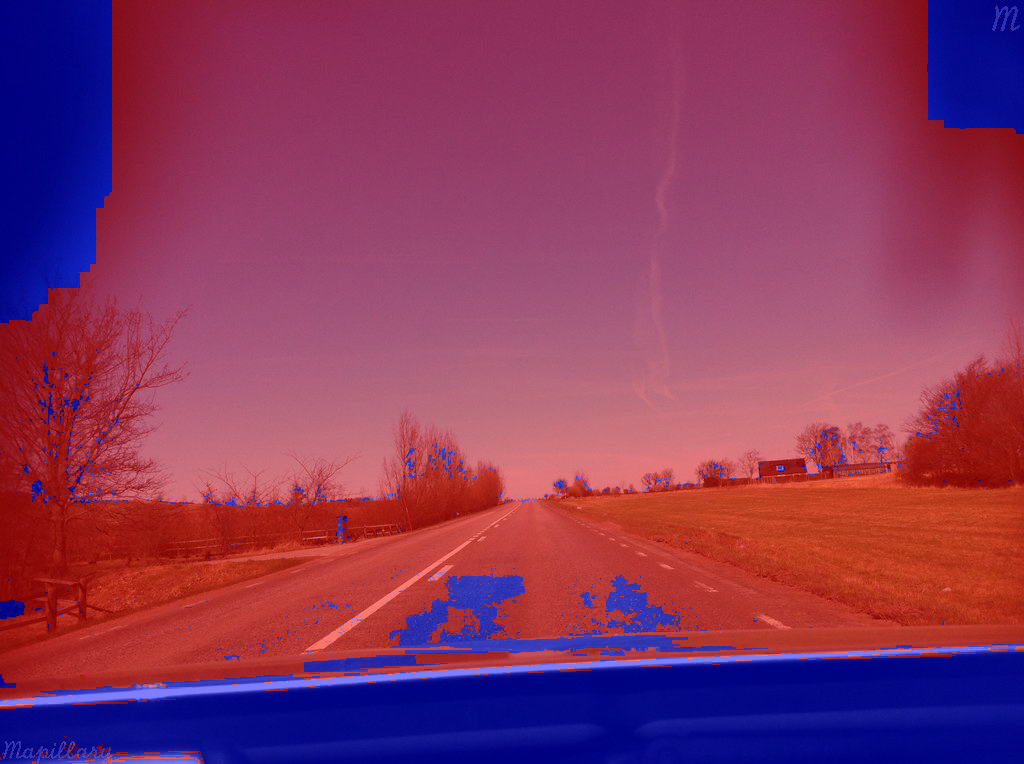
\includegraphics[width=0.45\textwidth]{result_15.png}
  \caption{Results on the image sequence \texttt{-ywLysPFu3TL85zOMOYJkw}}
	\label{fig:results}
\end{figure}



\section{Future works}
The experiments using method 3 show promising results.

To robustify the approaches:
\begin{enumerate}
\item Instead of pixels, use image patches and learn sparse dictionary of patches (see Julien Mairal PhD thesis). Discussion with Yubin about deep learning reminded me about this. I believe this would help a lot. Online learning is possible. Toolboxes in python should be available as well.
\item Perform histogram equalization for the sequence in case the illumination settings were very bad for taking pictures (cf. sequence key: \texttt{kDUGtZ3Nv6IkkmABg6hC8w})
\item Improve the way we update the regularization term?
\item Tune parameters to balance between data term and regularization term.
\item Update the priors with the last 5 segmentation results, instead of keeping all the history. For example, this will help to quickly adapt to sudden changes. I can think of a sudden illumination change because of the sun or, e.g., the windscreen wiper starts moving because of the rain.
\end{enumerate}


\subsection{Towards automatic detection of repeating patterns?}

We can compute temporal statistics in each pixel $p$ to determine the temporal mean color $\mu(p)$ and the temporal standard deviation $\sigma(p)$ from time step $t=1,\dots,N$. They are respectively shown in Fig. \ref{fig:mean_image} and Fig. \ref{fig:std_dev_image}.

The temporal standard deviation provides interesting cues but it seems hard to exploit as it is not sufficiently discriminative because of the streetview are also stationary, e.g. the sky, road.

\begin{figure}
	\centering
  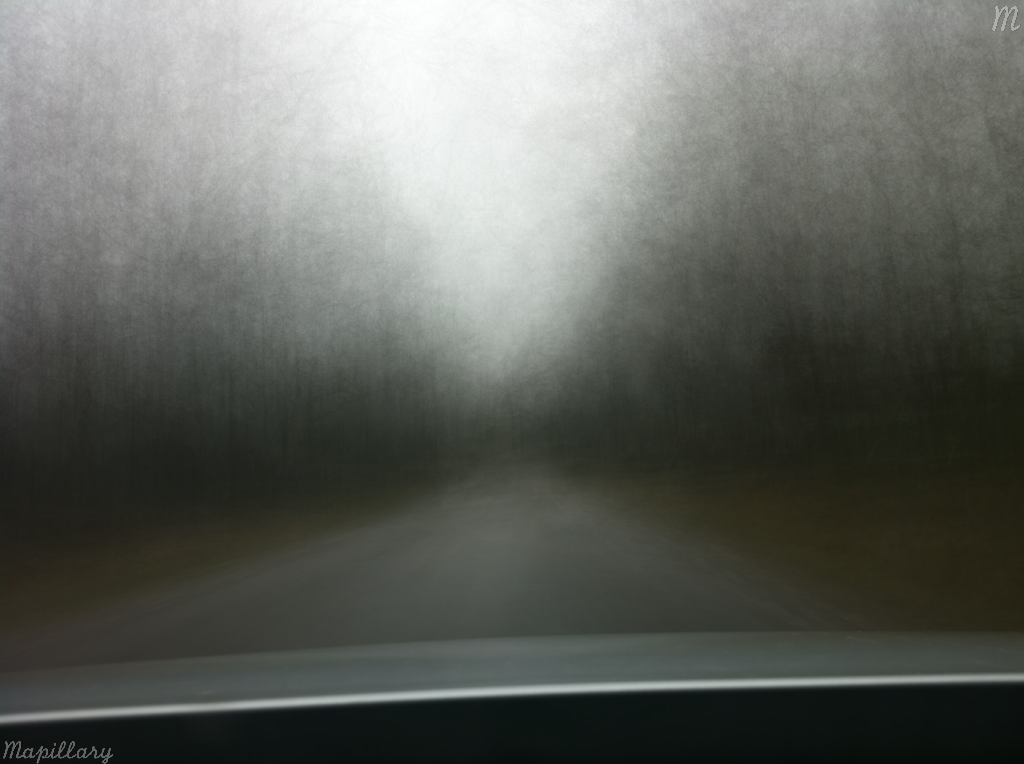
\includegraphics[width=0.8\textwidth]{mean_image.png}
	\caption{Temporal mean. Except the streetview, the car hood is relatively invariant over time.}
	\label{fig:mean_image}
\end{figure}

\begin{figure}
  \centering
  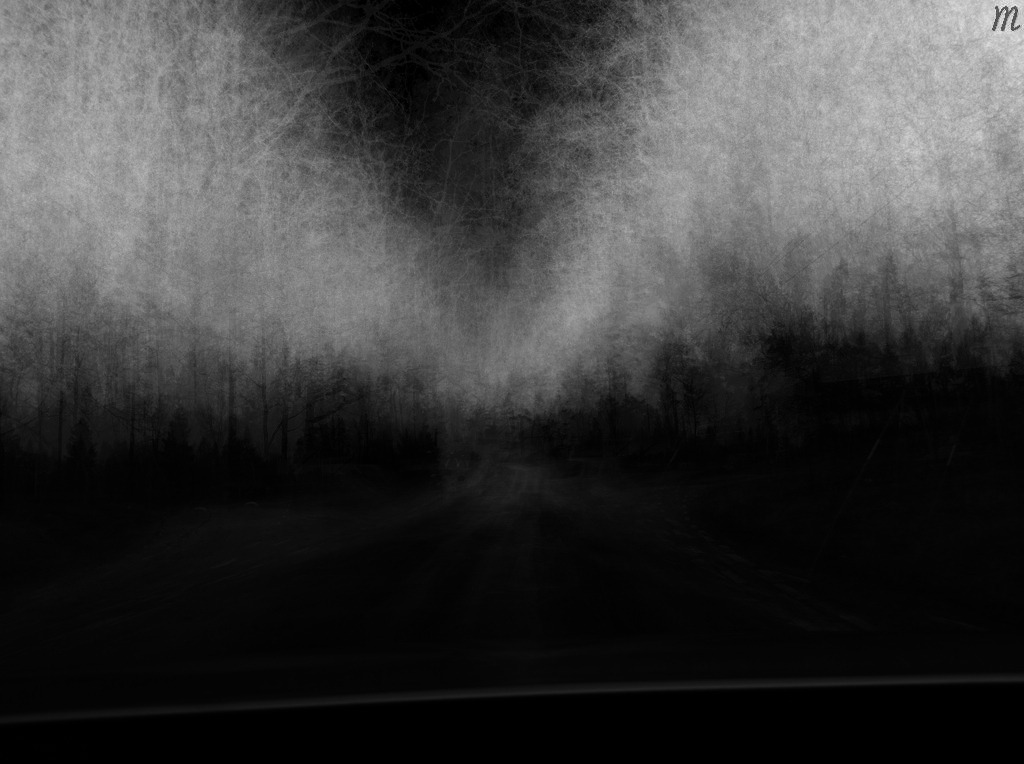
\includegraphics[width=0.8\textwidth]{std_dev_image.png}
	\caption{Temporal standard deviation. The whiter the pixel, the higher the standard deviation is. The trees are captured efficiently contrary to the road and the sky which are also stationary\dots.}
	\label{fig:std_dev_image}
\end{figure}

I write the idea of temporal statistics here as it may give rise to other ideas.


\section{Crop the image in 3:4 format that best fit the remaining good parts of the image.}

I will need more time. Leaving aside some heuristic methods, I have one idea that may be interesting.

Reusing the segmentation mask of each image, we want to find the largest rectangle $[x_1, x_2] \times [y_1, y_2]$ that maximizes the ratio between the number of streetview pixels and the number of uninteresting pixels.

Let us denote by $\rho(x_1, x_2, y_1, y_2)$ such ratio, i.e.:
\begin{equation}
\rho(x_1, x_2, y_1, y_2) \ = \  
\frac{
  \displaystyle
  \sum_{\substack{x_1 \leq x \leq x_2\\y_1 \leq y \leq y2}} \mathds{1}_{\{l(x,y)=1\}}
}
{
  \displaystyle
  \sum_{\substack{x_1 \leq x \leq x_2\\y_1 \leq y \leq y2}} \mathds{1}_{\{l(x,y)=0\}}
}
\end{equation}

The ratio can be computed very efficiently with integral images (cf. [Real-Time Face Detection, Viola and Jones, IJCV 2004]).

So finally, it means we want to solve the following problem
\begin{equation}
\begin{array}{cc}
\underset{x_1, x_2, y_1, y_2}{\text{maximize}} & \rho(x_1, x_2, y_1, y_2) + 
\displaystyle \frac{x_2-x_1}{w} + \displaystyle \frac{y_2-y_1}{h} \\
\text{subject to} & 
  \left\{
  \begin{array}{c}
    (y2-y1) = 3/4 (x_2 - x_1) \\
    0 \leq x1 \leq x_2 \leq W \\
    0 \leq y1 \leq y_2 \leq H \\
  \end{array}
  \right.
\end{array}
\end{equation}

Notice that the three terms $\rho(x_1, x_2, y_1, y_2)$, $\frac{x_2-x_1}{w}$ and $\frac{x_2-x_1}{w}$ are in $[0, 1]$. This means that we should not need to any weight to balance each of these terms.

The problem should be solvable efficiently by some branch-and-bound strategy. We may reuse some ideas from [Beyond Sliding Windows: Object Localization by Efficient Subwindow Search, Lampert et al. CVPR 2008].


\end{document}